\chapter{Matter Wave} % (fold)
\label{cha:Matter Wave}
    \section{The Pilot Wave of De Broglie}
        By 1920s scientists reliazed that Bohr theory had some issues
        \begin{itemize}
            \item It failed to predict of the observed intensities of the spectral lines.
            \item It had limited success in predicting emission and apsorption wavelengths for multielectron atoms.
            \item It failed to provide an equation of motion governing the time development of atomic systems starting from some initial state.
            \item It overemphasized the particle nature of amtter and could not explain the newly dicovered wave-particle duality of light.
            \item It did not supply a general scheme for "quantizing" other systems, especially those without periodic motion.
        \end{itemize}

        In 1923, Louis Victor de Broglie postulated that \textit{because photons have wave and particle characteristics, perhaps all forms of matter have wave 
        as well as particle properties}. According to him, electrons had a dual wave-particle nature.

        He found the the wavelength of a \textit{matter wave}
        \coloredeq{eq:de Broglie wavelength}{\lambda = \frac{h}{p} \qquad f=\frac{E}{h}}
        {\tiny \begin{itemize}
            \item $h$ is Planck's constant, 
            \item $p$ is the relativistic momentum
            \item $E$ is the total relativistic energy
        \end{itemize}}


        \paragraph{De Broglie's Explanation of Quantization in Bohr Model} % (fold)
        \label{par:De Broglie's Explanation of Quantization in Bohr Model}
        De Broglie applied the ideas of familiar wave properties such as standing wave and interference. He postulated that the electron as an standing wave bent aorund
        the nucleus with radius of Bohr orbit $r$. Thus only disceret set of wavelengths is allowed for standing waves.
        Amazingly, Bohr theory for quantization of angular momentum can be esaily explained by de Broglie's hypothesis: \textbf{the allowed Bohr orbits arise because the 
        electron matter waves interfere constructively when an integral number of wavelengths exactly fits into the circumference of a circle orbit}. Thus
        \begin{align}
            \label{eq:de Broglie hypothesis}
            n \lambda = 2 \pi r
        \end{align}
        where $r$ is the radius of the orbit. From Eq.\eqref{eq:de Broglie wavelength}, we have $\lambda=h/m_e v$, substituting this into Eq.\eqref{eq:de Broglie hypothesis}
        and solving for $L$, $m_e v r$
        \coloredeq{eq:de Broglie quantization}{m_e v r = n \hbar}
        which is exactly Bohr condition for quantization of angular momentum.
        % paragraph De Broglie's Explanation of Quantization in Bohr Model (end)

        \paragraph{The Davisson-Germer Experiment} % (fold)
        \label{par:The Davisson-Germer Experiment}
        In 1924, de Broglie had sugested that a stream of electrons traversing a small aperture shouls undergo diffraction phenomena. In 1925, Einstein was led to the need
        of postulating matter waves from an analysis of fluctuations of molecular gas. Also, he noted that a molecular beam should show a small diffraction effects.
        In 1927, the proof of the wave nature eas obtained by the work of Davisson and Germer, and George P. Thomson.

        \bulletpar Davisson-Germen's experiment was to understand the arrangement of atoms on the surface of a nickle sample by elastically scattering a beam of low-speed
        electrons from a polycrystalline nickle traget. They had three parameters that can be changed-- \textit{electron energy}; \textit{nickle target orientation}, 
        $\alpha$; and \textit{scatterin angle}, $\phi$.

        \bulletpar Their experiment was going normally, with constant electron energy of \SI{100}{eV}, the scattered intensity rapidly decreased as $\phi$ increased.
        Accidentally, someone dropped a flask of liquid air on the glass vacvum system, tearing the vaccum and oxidizing the nickle target, that had been in high
        temperature. To remove the oxide, they reduce the sample by heating it carefully in a flowing stream of hydrogen. After this reassembling, they found very
        different results: \textit{Strong variations in the intensity of scattered electrons with angle}.

        \bulletpar This heating annealed the nickle target, causing large single-crystal regions to develop in the polycrystalline sample. These crystalline regions 
        provided the extended regualr lattice needed to observe electron diffraction. Davisson and Germen relized that it was the elastic scattering from \textit{single
        crystals} that produced such unusual results. 

        \bulletpar The idea is that they calculated the eavelength of the electrons from simple diffraction formula and compared it with de Broglie's formula.
        Thus, for an electron we have 
        \begin{align*}
            \frac{1}{2}m_e v^2 = eV
        \end{align*}
        Substitute $v$ into de Broglie relation
        \begin{align*}
            \lambda = \frac{h}{m_e v} = \frac{h}{\sqrt{2Vem_e}}
        \end{align*}
        Also, the the wavelength csn be obtainde by considering the nickle atoms to be a reflaction diffraction grating. Only the atoms at the surface is considere, since
        x-rays cannot penetrate deeply into crystal. Thus to find the constructive interference we have 
        \begin{align}
            d \sin{\phi} = n \lambda
        \end{align}
        The diffraction lines from high-energy electrons are so sharp, and these electron can penetrate deeper in the crystal. As result, we need to use Bragg's law instead.

        \bulletpar Davisson and Germen concluded that this wavelength agrees very well with that from de Broglie's formula, confirming the electron matter wave. If de Broglie's 
        postulate is true for all matter, then any objects with mass $m$ has wavelike property.
        % paragraph The Davisson-Germer Experiment (end)

        \paragraph{The Electron Microdcope} % (fold)
        \label{par:The Electron Microdcope}
        The ability of controlling electron eavelength, even shorther than the visible light, provide us with a great tool investigate small objects.
        First \textbf{transmission electron microscope} (TEM), was built by Max Knoll and Ernst Ruska in 1931; it focuses electron beams accelerated by \SI{100}{kV}
        with magnetic lenses
        and creates a flta-looking two-dimensional shadow pattern on its screen, the resultof varying degrees of electron transmission through the object.
        
        \bulletpar magnificationAn optical microscope using ultraviolet has a maginification of 2000 and resolving power of \SI{100}{nm}. TEM can reach a magnification of \num{1000000}
        and resolving power of \SI{0.2}{nm}

        \bulletpar A second type of electron microscope with less resolution and magnification than TEM, but capable of producing three-dimensional images, is
        called \textbf{scanning electron microscope} (SEM).
        % paragraph The Electron Microdcope (end)

    \section{Wave Groups and Dispersion}
        The matter eave of a moving particle has a large probability to be found in a small region of space only at a specific time. Hence, the traveling 
        sinusoidal matter wave od finite extent and constant amplitude cannot represent a localized moving particle.

        \bulletpar Thus we need to introduce a pulse or a \textbf{wave group} of limited spatial extent. This pulse can be found by adding up sinusiodal wave with 
        different wavelengths. The resulting wave group will have a \textbf{group apeed} $v_g$ identical to the classical particle speed.

        \begin{wrapfigure}{r}{0.25\linewidth}
            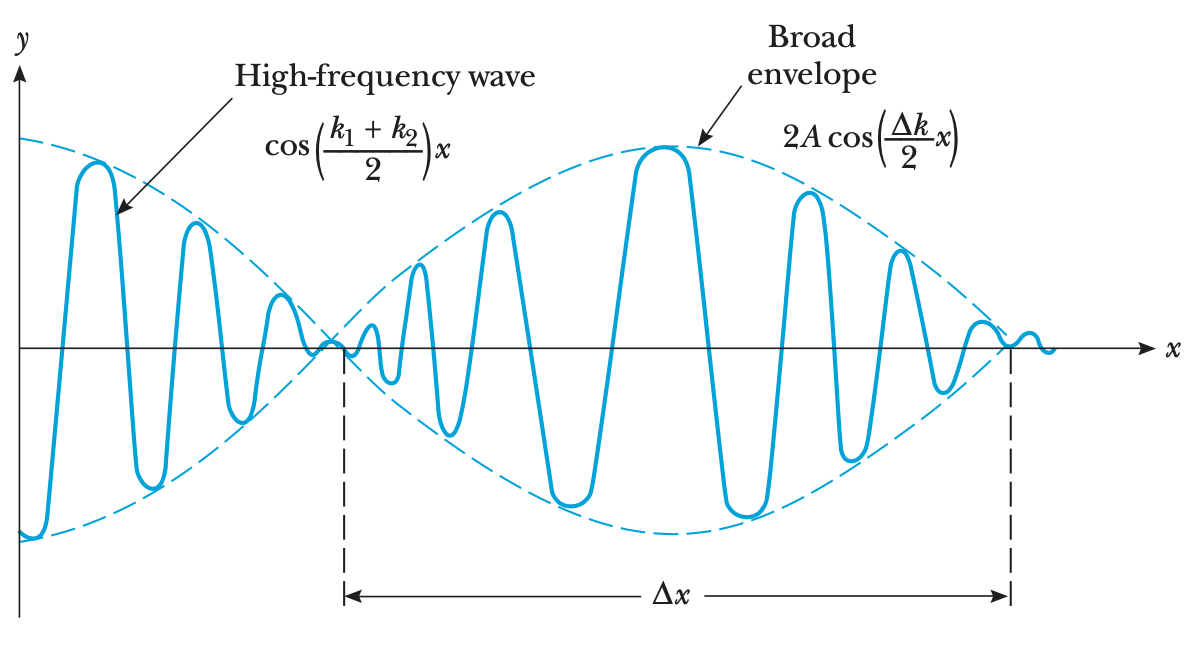
\includegraphics[width=0.9\linewidth]{figures/group-wave.png}
            \label{fig:wave group}
            \caption{A wave group}
        \end{wrapfigure}

        \bulletpar In fact, all observed waves are limited to definite regions of space and are called \textit{pulses}, \textit{eave groups}, or \textit{eave 
        pachets} in matter waves. A plane wave with an exact wavelength and an infinite extension is an abtraction. Water waves, light waves, waves along a string,
        and sound wave all must be modeled by a group wave.

        \starpar A \textbf{wave group} consists of a superposition of waves with \textit{different wavelengths}, with the amplitude and phase of each component
        wave adjusted to make a constructive interference over a small region of space. A good example is the beats in sound waves.

        \bulletpar Consider a one=dimensional wave propagating in the positive $x$ direction with a \textbf{phase speed} $v_p$. This traveling wave with 
        wavelength $\lambda$ and frequenct $f$, and amplitude $A$ is written like 
        \begin{align}
            \label{eq:wave group:1}
            y = A \cos{\left( \frac{2 \pi}{\lambda} - 2 \pi ft \right)} \qquad \text{and} \quad v_p = \Lambda f
        \end{align}
        take $\omega = 2 \pi f$ (\textit{angular frequency}) and $k=2 \pi/\Lambda$ (\textit{wavenumber}), thus 
        \begin{align}
            \label{eq:wave group:2}
            y = A \cos{(k x - \omega t)}
        \end{align}
        and the the \textit{phase velocity}
        \coloredeq{eq:group velocity}{v_p = \frac{\omega}{k} }

        \bulletpar Let us form a superposition of two waves having the same amplitude and treavleing in the positive $x$, but different in wavelength, frequency, 
        and phase velocities. Hence,
        \begin{align}
            \label{eq:wave group:3}
            y = y_1 + y_2 = A \cos{(k_1 x - \omega_1 t)} + \cos{(k_2 x - \omega_2 t)}
        \end{align}
        Using the trigonometric identity: $\cos{a} + \cos{b} = 2\, \cos{\frac{1}{2}(a-b)} \cos{\frac{1}{2}(a+b)}$, we get 
        \begin{align}
            \label{eq:wave group:4}
            y = 2A \cos{\frac{1}{2}\left[ (k_2-k_1)x - (\omega_2-\omega_1)t \right]} \cos{\frac{1}{2} \left[(k_1+k_2)x - (\omega_1+\omega_2)t \right]}
        \end{align}
        For case of two waves with slightly different values of $k$ and $\omega$, we see that $\Delta{k} = k_2-k_1$ $\Delta{\omega} = \omega_2-\omega_1$ represent 
        small wave, but $(k_1+k_2)$ and $(\omega_1 + \omega_2)$ represent larger wave. So we can say that Eq.\eqref{eq:wave group:4} has a broad sinusoidal 
        \underline{envelope}, 
        \begin{align}
            \label{eq:wave group:5}
            2A \cos{\left( \frac{\Delta{k}}{2}x - \frac{\Delta{\omega}}{2}t \right)}
        \end{align}
        modulating a high-frequency wave within the envelope
        \begin{align}
            \label{eq:wave group:6}
            \cos{\left( \frac{k_1+k_2}{2}x - \frac{\omega_1+\omega_2}{2}t \right)}
        \end{align}
        This superposition is shown in Fig.\eqref{fig:wave group}. We can find the speed of the high-frequency wave and the envelope wave by dividing the 
        coefficient of $t$ by the one of $x$,
        \begin{align}
            \label{eq:wave group:7}
            v_p = \frac{(\omega_1+\omega_2)/2}{(k_1+k_2)/2} \approx \frac{\omega_1}{k_1} = v_1
        \end{align}
        and for the envelope velocity
        \begin{align}
            \label{eq:wave group:7}
            v_g = \frac{\Delta{\omega}}{\Delta{k}}
        \end{align}

        \bulletpar A general characteristic of wave groups is that both is a linited duration in time, $\Delta{t}$, and a limited extent in space, $\Delta{x}$.
        Thus the smaller the spatial width of the pulse, $\Delta{x}$, the larger the range od wavelengths or wavenumbers, $k$,
        \begin{align}
            \label{eq:wave group:8}
            \Delta{x} \Delta{k} \approx 1
        \end{align}
        Likwise, the smaller the temporal duration, $\Delta{t}$, the larger the frequencies, $\omega$
        \begin{align}
            \label{eq:wave group:9}
            \Delta{t} \Delta{\omega} \approx 1
        \end{align}
        In electronics, this condition is called \textit{response time-bandwidth formula}.

        \starpar \textbf{Both $\Delta{x}$ and $\Delta{k}$ cannot become arbitrarily small, but as one decreases the other must increase}. Our simple two-wave 
        model can show the general principle given by Eq.\eqref{eq:wave group:8} and Eq.\eqref{eq:wave group:9}. Let the spatial extent of our group be the 
        distance between two adjacent minima ($y=0$), labeled $\Delta{x}$ in Fig.\eqref{fig:wave group} we find from the envelope term: 
        $2A \cos{(\frac{1}{2}\Delta{kx})}$, then $\frac{1}{2} \Delta{k} \Delta{x}=\pi$
        \begin{align}
            \label{eq:wave group:10}
            \Delta{k} \Delta{x} = 2 \pi
        \end{align}
        where $\Delta{k} = k_2 - k_1$ is the present wavenumbers. Similarly, if we hold $x$ constant and changing $t$, we have 
        $\frac{1}{2}(\omega_2-\omega_1)\Delta{t} = \pi$, 
        \begin{align}
            \label{eq:wave group:11}
            \Delta{\omega} \Delta{t} = 2 \pi
        \end{align}
        as result we see that Eq.\eqref{eq:wave group:10} and Eq.\eqref{eq:wave group:11} agree with the \textit{general principles}. 

        \bulletpar The addition of two waves with discrete frequencies is informative, but produces an infinite wave instead of a true pulse. Im general, many waves 
        having a continuous distribuation of wavelengths must be added to form a packet, finite over a limited range. In this case, the Eq.\eqref{eq:wave group:7},
        for \textbf{group velocity} becomes, 
        \coloredeq{eq:group velocity}{
            v_g = \frac{d\omega}{dk} \Big|_{k_0}
        }
        where $k_0$ is the centeral wavenumber of the many waves present. We can find a connection bewtween the group velocity and the phase velocity, if 
        $\omega = k v_p$ then,
        \begin{align}
            \label{eq:group and phase velovity}
            v_g = \frac{d\omega}{dk} \Big|_{k_0} = v_p \Big|_{k_o} + k \frac{dv_p}{dk} \Big|_{k_0}
        \end{align}

        \bulletpar \textbf{Dispersion} happens in materials in which the \textit{phase velocity} changes with wavelength.



% chapter Matter Wave (end)